%%%%%%%%%%%%%%%%%%%%%%%%%%%%%%%%%%%%%%%%%%%%%%%%%%%%%%%%%%%%%%%%%%%%%%%%%%%%%%%
\documentclass[hyperref={pdfpagelabels=false},compress,table]{beamer} % 在Mac下无法编译
% \documentclass[compress,table]{beamer} % 在Mac下使用
% package for font
\usepackage{fontspec}
\defaultfontfeatures{Mapping=tex-text}  %%如果没有它,会有一些 tex 特殊字符无法正常使用,比如连字符。
\usepackage{xunicode,xltxtra}
\usepackage[BoldFont,SlantFont,CJKnumber,CJKchecksingle]{xeCJK}  % \CJKnumber{12345}: 一万二千三百四十五
\usepackage{CJKfntef}  %%实现对汉字加点、下划线等。
\usepackage{pifont}  % \ding{}
% package for math
\usepackage{amsfonts}

% package for graphics
\usepackage[americaninductors,europeanresistors]{circuitikz}
\usepackage{tikz}
\usetikzlibrary{plotmarks}  % placements=positioning
\usepackage{graphicx}  % \includegraphics[]{}
\usepackage{subfigure}  %%图形或表格并排排列
% package for table
\usepackage{colortbl,dcolumn}  %% 彩色表格
\usepackage{multirow}
\usepackage{multicol}
\usepackage{booktabs}
% package for code
\usepackage{fancyvrb}
\usepackage{listings}

% \usepackage{animate}
% \usepackage{movie15}

%%%%%
% setting for beamer
\usetheme{default} % Madrid(常用), Copenhagen, AnnArbor, boxes(白色), Frankfurt,Berkeley
\useoutertheme[subsection=true]{miniframes} % 使用Berkeley时注释本行
\usecolortheme{sidebartab}
\usefonttheme{serif}  %%英文使用衬线字体
% \setbeamertemplate{background canvas}[vertical
% shading][bottom=white,top=structure.fg!7] %%背景色,上25%的蓝,过渡到下白。
\setbeamertemplate{theorems}[numbered]
\setbeamertemplate{navigation symbols}{}  %% 去掉页面下方默认的导航条
\setbeamercovered{transparent}  %设置 beamer 覆盖效果

% 设置标题title背景色
% \setbeamercolor{title}{fg=black, bg=lightgray!60!white}
\setbeamercolor{title}{fg=white, bg=black!70!white}

% 设置每页小LOGO
\pgfdeclareimage[width=1cm]{ouc}{figures/static/ouc.pdf}
\logo{\pgfuseimage{ouc}{\vspace{-20pt}}}

% setting for font
%%\setCJKmainfont{Adobe Kaiti Std}
\setCJKmainfont{SimSun} 
%% \setCJKmainfont{FangSong_GB2312} 
%% \setmainfont{Apple Garamond}  %%苹果字体没有SmallCaps
\setCJKmainfont{SimSun} 
%FUNNY%\setCJKmainfont{DFPShaoNvW5-GB}  %%华康少女文字W5(P)
%FUNNY%\setCJKmainfont{FZJingLeiS-R-GB}  %%方正静蕾体
%FUNNY%\setmainfont{Purisa}
%\setsansfont[Mapping=tex-text]{Adobe Song Std}
     %如果装了Adobe Acrobat,可在font.conf中配置Adobe字体的路径以使用其中文字体。
     %也可直接使用系统中的中文字体如SimSun、SimHei、微软雅黑等。
     %原来beamer用的字体是sans family;注意Mapping的大小写,不能写错。
     %设置字体时也可以直接用字体名,以下三种方式等同:
     %\setromanfont[BoldFont={黑体}]{宋体}
     %\setromanfont[BoldFont={SimHei}]{SimSun}
     %\setromanfont[BoldFont={"[simhei.ttf]"}]{"[simsun.ttc]"}
% setting for graphics
\graphicspath{{figures/}}  %%图片路径
\renewcommand\figurename{图}

% setting for pdf
\hypersetup{% pdfpagemode=FullScreen,%
            pdfauthor={Xiaodong Wang},%
            pdftitle={Title},%
            CJKbookmarks=true,%
            bookmarksnumbered=true,%
            bookmarksopen=false,%
            plainpages=false,%
            colorlinks=true,%
            citecolor=green,%
            filecolor=magenta,%
            linkcolor=blue,%red(default)
            urlcolor=cyan}

% setting for fontspec
\XeTeXlinebreaklocale "zh"  %%表示用中文的断行
\XeTeXlinebreakskip = 0pt plus 1pt minus 0.1pt  %%多一点调整的空间
%%%%%

% font setting by xeCJK
\setCJKfamilyfont{NSimSun}{NSimSun}
\newcommand{\song}{\CJKfamily{NSimSun}}
%%%\setCJKfamilyfont{AdobeSongStd}{Adobe Song Std}
%%%\newcommand{\AdobeSong}{\CJKfamily{AdobeSongStd}}
\setCJKfamilyfont{FangSong}{FangSong_GB2312}
\newcommand{\fang}{\CJKfamily{FangSong}}
%%%\setCJKfamilyfont{AdobeFangsongStd}{Adobe Fangsong Std}
%%%\newcommand{\AdobeFang}{\CJKfamily{AdobeFangsongStd}}
\setCJKfamilyfont{SimHei}{SimHei}
\newcommand{\hei}{\CJKfamily{SimHei}}
%%%\setCJKfamilyfont{AdobeHeitiStd}{Adobe Heiti Std}
%%%\newcommand{\AdobeHei}{\CJKfamily{AdobeHeitiStd}}
\setCJKfamilyfont{KaiTi}{KaiTi}
\newcommand{\kai}{\CJKfamily{KaiTi}}
%%%\setCJKfamilyfont{AdobeKaitiStd}{Adobe Kaiti Std}
\newcommand{\AdobeKai}{\CJKfamily{AdobeKaitiStd}}
\setCJKfamilyfont{LiSu}{LiSu}
\newcommand{\li}{\CJKfamily{LiSu}}
\setCJKfamilyfont{YouYuan}{YouYuan}
\newcommand{\you}{\CJKfamily{YouYuan}}
\setCJKfamilyfont{FZJingLei}{FZJingLeiS-R-GB}
\newcommand{\jinglei}{\CJKfamily{FZJingLei}}
\setCJKfamilyfont{MSYH}{Microsoft YaHei}
\newcommand{\msyh}{\CJKfamily{MSYH}}

% 自定义颜色
\def\Red{\color{red}}
\def\Green{\color{green}}
\def\Blue{\color{blue}}
\def\Mage{\color{magenta}}
\def\Cyan{\color{cyan}}
\def\Brown{\color{brown}}
\def\White{\color{white}}
\def\Black{\color{black}}

\lstnewenvironment{xmlCode}[1][]{% for Java
  \lstset{
    basicstyle=\tiny\ttfamily,%
    columns=flexible,%
    framexleftmargin=.7mm, %
    % frame=shadowbox,%
    % rulesepcolor=\color{cyan},%
     frame=single,%
    backgroundcolor=\color{white},%
    xleftmargin=4\fboxsep,%
    xrightmargin=4\fboxsep,%
    numbers=left,numberstyle=\tiny,%
    numberblanklines=false,numbersep=7pt,%
    language=xml, %
    }\lstset{#1}}{}

\lstnewenvironment{javaCode}[1][]{% for Java
  \lstset{
    basicstyle=\tiny\ttfamily,%
    columns=flexible,%
    framexleftmargin=.7mm, %
    frame=shadowbox,%
    rulesepcolor=\color{cyan},%
    % frame=single,%
    backgroundcolor=\color{white},%
    xleftmargin=4\fboxsep,%
    xrightmargin=4\fboxsep,%
    numbers=left,numberstyle=\tiny,%
    numberblanklines=false,numbersep=7pt,%
    language=Java, %
    }\lstset{#1}}{}

\lstnewenvironment{shCode}[1][]{% for Java
  \lstset{
    basicstyle=\scriptsize\ttfamily,%
    columns=flexible,%
    framexleftmargin=.7mm, %
    frame=shadowbox,%
    rulesepcolor=\color{brown},%
    % frame=single,%
    backgroundcolor=\color{white},%
    xleftmargin=4\fboxsep,%
    xrightmargin=4\fboxsep,%
    numbers=left,numberstyle=\tiny,%
    numberblanklines=false,numbersep=7pt,%
    language=sh, %
    }\lstset{#1}}{}

\newcommand\ask[1]{\vskip 4bp \tikz \node[rectangle,rounded corners,minimum size=6mm,
  fill=white,]{\Cyan \includegraphics[height=1.5cm]{question} \Large \msyh #1};}

\newcommand\wxd[1]{\vskip 4bp \tikz \node[rectangle,minimum size=6mm,
  fill=blue!60!white,]{\White \ding{118} \msyh #1};}

\newcommand\xyy[1]{\vskip 2bp \tikz \node[rectangle,minimum size=3mm,
  fill=black!80!white,]{\White \msyh\scriptsize #1};}

\newcommand\cxf[1]{\vskip 4bp \tikz \node[rectangle,rounded corners,minimum size=6mm,
  fill=orange!60!white,]{\White \ding{42} \msyh #1};}

\newcommand\samp[1]{\vskip 2bp \tikz \node[rectangle,minimum size=3mm,
  fill=white!100!white,]{\Mage\msyh \small CODE \ding{231} \Black #1};\vskip -8bp}

\newcommand\zhyfly[1]{\tikz \node[rectangle,rounded corners,minimum size=6mm,ball color=red!25!blue,text=white,]{#1};}

\setbeamerfont{frametitle}{series=\msyh} % 修改Beamer标题字体

\makeatletter
\newcommand{\Extend}[5]{\ext@arrow 0099{\arrowfill@#1#2#3}{#4}{#5}}
\makeatother


%%%%%%%%%%%%%%%%%%%%%%%%%%%%%%%%%%%%%%%%%%%%%%%%%%%%%%%%%%%%%%%%%%%%%%%%%%%%%%%
% \titlepage
\title[KevinW@OUC]{\hei {\huge Java 应用与开发}\\  
  Java GUI编程}
\author[王晓东]{王晓东\\
  \href{mailto:wangxiaodong@ouc.edu.cn}{\footnotesize wangxiaodong@ouc.edu.cn}}
\institute[中国海洋大学]{\small 中国海洋大学}
\date{\today}
\titlegraphic{\vspace{-6em}
\includegraphics[height=6cm]{static/ouc.pdf}\vspace{-6em}}
%%%%%
\begin{document}
%% Delete this, if you do not want the table of contents to pop up at
%% the beginning of each subsection:
\AtBeginSection[]{                              % 在每个Section前都会加入的Frame
  \frame<handout:0>{
    \frametitle{\textbf{\hei 接下来…}}
    \tableofcontents[currentsection]
  }
}  %

\AtBeginSubsection[]                            % 在每个子段落之前
{
  \frame<handout:0>                             % handout:0 表示只在手稿中出现
  {
    \frametitle{\textit{\hei 接下来…}}\small
    \tableofcontents[current,currentsubsection] % 显示在目录中加亮的当前章节
  }
}
\frame{\titlepage}
%%%%%%%%%%%%%%%%%%%%%%%%%%%%%%%%%%%%%%%%%%%%%%%%
\begin{frame}
  \frametitle{学习目标}
  \begin{enumerate}
  \item 了解用Java开发桌面软件图形用户界面的常用工具集
  \item 掌握AWT的常用组件和视觉控制
  \item 深入理解GUI事件处理机制
  \item 了解Applet,特别是其历史渊源,了解与Applet类似的技术
  \item 理解Swing和AWT的关系,学习使用Swing的典型组件构建较复杂的图形界面程序
  \end{enumerate}  
\end{frame}

\section*{大纲}
\frame{\frametitle{大纲} \tableofcontents }


\begin{frame}[fragile]
  \frametitle{用Java构建图形界面,我们有什么选择?}

  \begin{itemize}
  \item AWT
  \item Swing
  \item Java FX
  \item 多语言混合开发
  \end{itemize}
\end{frame}

\section{GUI组件及布局}

\begin{frame}[fragile] % [fragile]参数使得能够插入代码
  \frametitle{概念和术语}

  \tta{图形用户界面}

  GUI (Graphical User Interface),Java主要分为AWT和Swing两大系列GUI API。

  \tta{抽象窗口工具集}

  AWT (Abstract Window Toolkit)

  \tta{相关软件包}

  \begin{description}
  \item[java.awt包] 提供基本GUI组件、视觉控制和绘图工具API。
  \item[java.awt.event包] 提供Java GUI事件处理API。
  \end{description}
\end{frame}

\begin{frame}[fragile] % [fragile]参数使得能够插入代码
  \frametitle{组件和容器}
  
  \begin{block}{组件}
    组件(Component)是图形用户界面的基本组成元素,凡是能够以图形化方式显示在屏幕上并能够与
    用户进行交互的对象均为组件,如菜单、按钮、标签、文本框、滚动条等。
  \end{block}

  \pause
  
  \begin{itemize}[<+-|alert@+>]\kai
  \item 组件不能独立地显示出来,必须将组件放在一定的容器中才可以显示出
    来。
  \item JDK的java.awt包中定义了多种GUI组件类,
    如Menu、Button、Label、TextField等。
  \item 抽象类java.awt.Component是除菜单相关组件之外所有Java AWT组件类
    的根父类,该类规定了GUI组件的基本特性,如尺寸、位置和颜色效果等,并
    实现了作为一个GUI部件所应具备的基本功能。
  \item java.awt.MenuComponent是所有与菜单相关的组件的父类。
  \end{itemize}
\end{frame}

\begin{frame}[fragile] % [fragile]参数使得能够插入代码
  \frametitle{组件和容器}
  
  \begin{block}{容器}
    容器(Container)实际上是Component的子类,容器类对象本身也是一个组
    件,具有组件的所有性质,另外还具有容纳其它组件和容器的功能。容器类
    对象可使用方法add()添加组件。
  \end{block}

  \pause
  
  \ttc{两种主要的容器类型}
  
  \begin{description}\kai
  \item[\fbox{java.awt.Window}] 可自由停泊的顶级窗口。
  \item[\fbox{java.awt.Panel}] 可作为容器容纳其他组件,但不能独立存在,必须被添加到其他容
    器(如Frame)中。
  \end{description}
\end{frame}

\begin{frame}[fragile] % [fragile]参数使得能够插入代码
  \frametitle{常用的组件和容器 \ding{182}}

  \begin{table}
    \scriptsize
    \setlength{\extrarowheight}{1.2mm}
    \rowcolors[]{1}{blue!30}{blue!10}
    \begin{tabular}{lll}
      {\bf 组件类型} & {\bf 父类}  & {\bf 说明}\\
      Button & Component & 可接收点击操作的矩形GUI组件\\
      Canvas & Component & 用于绘图的面板\\
      Checkbox & Component & 复选框组件\\
      CheckboxMenuItem & MenuItem & 复选框菜单项组件\\
      Choice & Component & 下拉式列表框,内容不可改变\\
      Component & Object & 抽象的组件类\\
      Container & Component & 抽象的容器类\\
      Dialog & Window & 对话框组件,顶级窗口、带标题栏\\
      FileDialog & Dialog & 用于选择文件的平台相关对话框\\
      Frame & Window & 基本的Java GUI窗口组件\\
      Label & Component & 标签类\\
    \end{tabular}
  \end{table}
\end{frame}

\begin{frame}[fragile] % [fragile]参数使得能够插入代码
  \frametitle{常用的组件和容器 \ding{183}}

  \begin{table}
    \scriptsize
    \setlength{\extrarowheight}{1.2mm}
    \rowcolors[]{1}{blue!30}{blue!10}
    \begin{tabular}{lll}
      {\bf 组件类型} & {\bf 父~类}  & {\bf 说~明}\\
      List & Component & 包含内容可变的条目的列表框组件\\
      MenuBar & MenuComponent & 菜单条组件\\
      Menu & MenuItem & 菜单组件\\
      MenuItem & MenuComponent & 菜单项组件\\
      Panel & Container & 基本容器类,不能单独停泊\\
      PopupMenu & Menu & 弹出式菜单组件\\
      Scrollbar & Component & 滚动条组件\\
      ScrollPane & Container & 带水平及垂直滚动条的容器组件\\
      TextComponent & Component & TextField和TextArea的基本功能\\
      TextField & TextComponent & 单行文本框\\
      TextArea & TextComponent & 多行文本域\\
      Window & Container & 抽象的GUI窗口类,无布局管理器\\
    \end{tabular}
  \end{table}
\end{frame}

\begin{frame}[fragile] % [fragile]参数使得能够插入代码
  \frametitle{Frame类}

  Frame类的显示效果是一个标准的图形窗口,它封装了GUI组件的各种属性信息,如尺寸、可见性等。

  \pause
  
  \begin{enumerate}\kai
  \item Frame对象的显示效果是一个可自由停泊的顶级“窗口”,带有标题和尺寸重置角标。
  \item Frame默认初始化为不可见的,可以调用Frame对象的setVisible(true)方法使之变为可见。
  \item 作为容器Frame还可使用add()方法包含其他组件。
  \end{enumerate}

  \codeset{sample.awt.FrameSample.java}
\end{frame}


\begin{frame}[fragile] % [fragile]参数使得能够插入代码
  \frametitle{组件定位}

  Java组件在容器中的定位由{\hei 布局管理器}决定。如要人工控制组件在容器中的定位,可取
  消布局管理器,然后使用Component类的下述成员方法设置:

  \begin{columns}
    \column{0.3\textwidth}
    \begin{itemize}
    \item setLocation()
    \item setSize()
    \item setBounds()
    \end{itemize}

    \column{0.8\textwidth}
    \begin{figure}
      \centering
      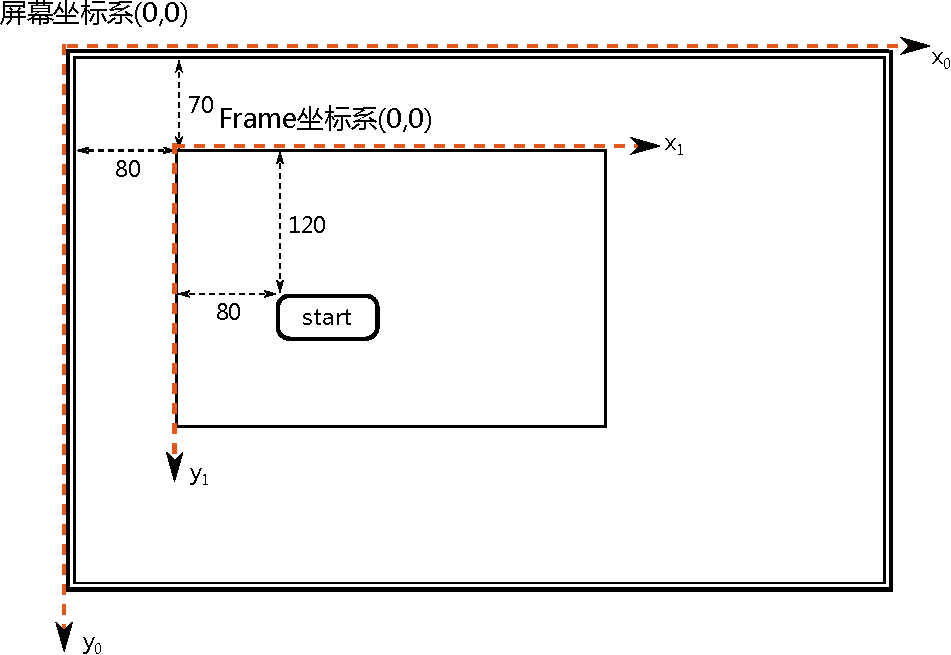
\includegraphics[width=1.0\textwidth]{fig02.pdf}
    \end{figure}
  \end{columns}

\end{frame}

\begin{frame}[fragile] % [fragile]参数使得能够插入代码
  \frametitle{Panel类}

  \begin{itemize}
  \item Panel提供容纳组件的空间。
  \item Panel不能独立存在,必须被添加到其他容器中。
  \item 可以采用和所在容器不同的布局管理器。
  \end{itemize}
  \codeset{sample.awt.FrameWithPanelSample.java}
\end{frame}

\begin{frame}[fragile] % [fragile]参数使得能够插入代码
\frametitle{布局管理器}

容器对其中所包含组件的排列方式,包括组件的位置和大小设定,被称为容器的布局(Layout)。

为了使图形用户界面具有良好的平台无关性,Java语言提供了布局管理器来管理容器的布局,而不建
议直接设置组件在容器中的位置和尺寸。

\ttc{布局管理器类层次}
{\small 
\begin{verbatim}
 LayoutManager----FlowLayout  
             |
             +----GridLayout

LayoutManager2----BorderLayout
             |
             +----CardLayout
             |
             +----GridBagLayout
\end{verbatim}}
注:LayoutManager2是LayoutManager的子接口。
\end{frame}

\begin{frame}[fragile] % [fragile]参数使得能够插入代码
  \frametitle{布局管理器}
  \begin{itemize}
  \item 每个容器都有一个布局管理器,当容器需要对某个组件进行定位或判断其大小尺寸时,就会调
    用其对应的布局管理器。
  \item 可以在容器创建后调用其setLayout()方法设置其布局管理器类型。
  \item Container类型容器没有默认的布局管理器,即其layoutMgr属性为null,在其子类中才进行分
    化。
  \end{itemize}
  \ttc{默认的布局管理器}
  \begin{figure}
    \centering
    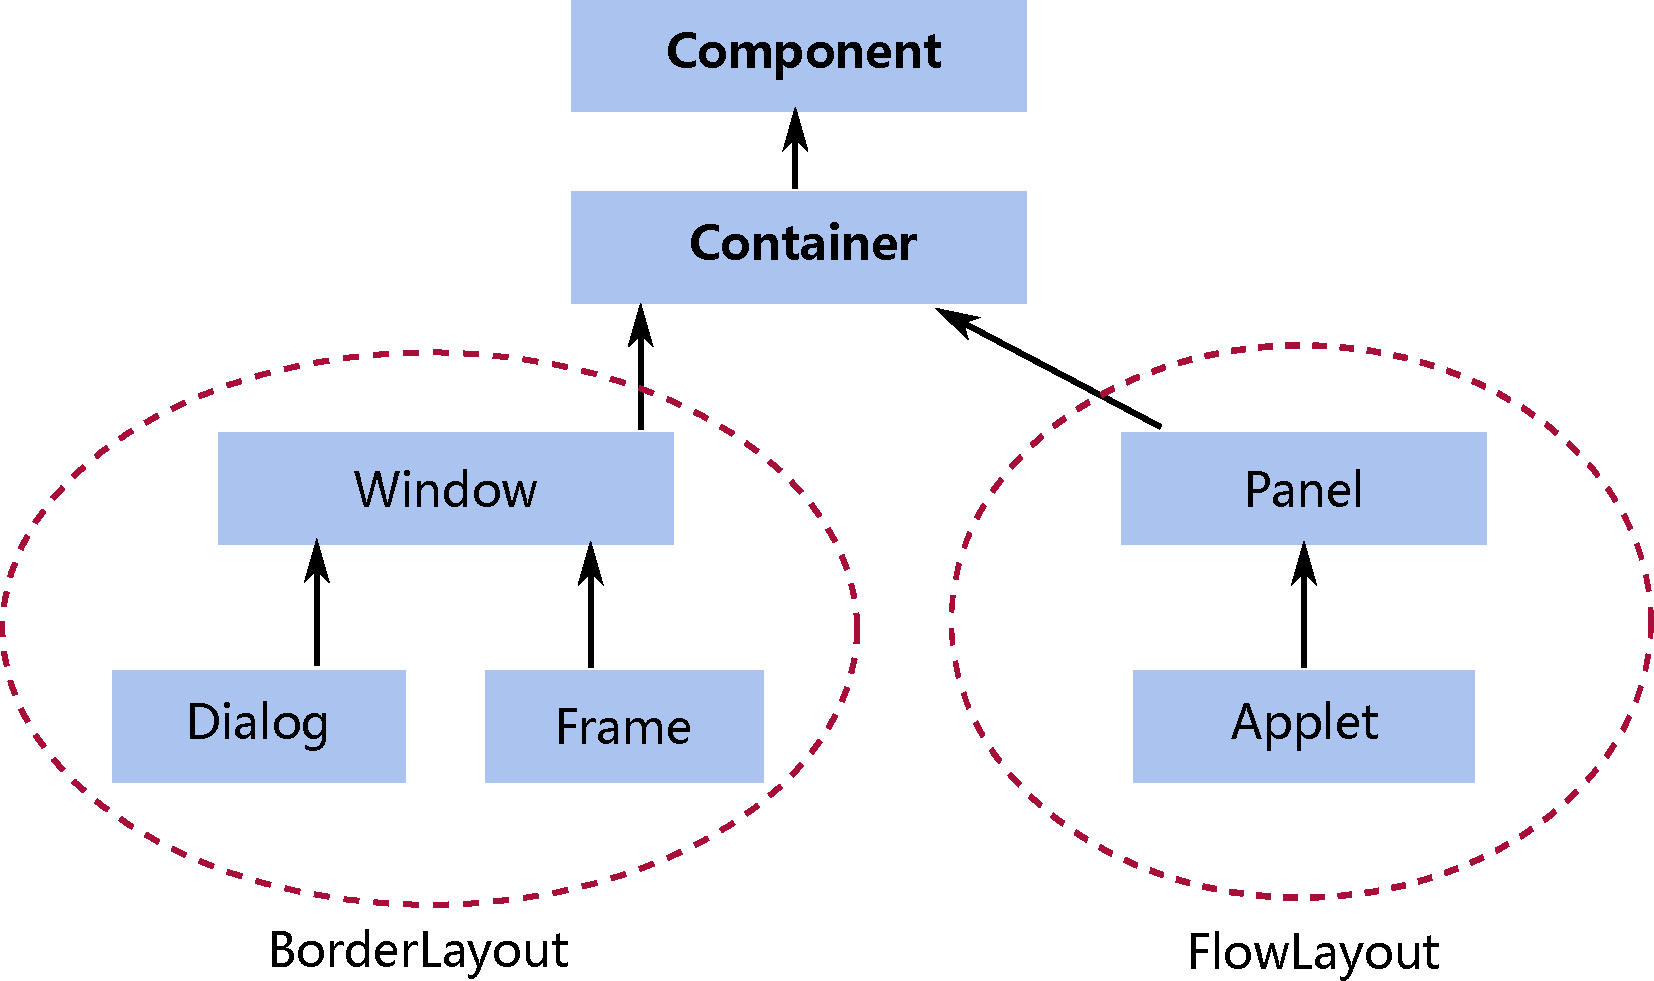
\includegraphics[width=0.6\textwidth]{fig04.pdf}
  \end{figure}
\end{frame}

\begin{frame}[fragile] % [fragile]参数使得能够插入代码
  \frametitle{FlowLayout}

  \tta{流式布局} \\是Panel(及其子类)类型容器的默认布局管理器类型。

  \tta{布局效果}
  \begin{itemize}\kai
  \item 组件在容器中按照加入次序逐行定位,行内从左到右,一行排满后换行。
  \item 不改变组件尺寸,即按照组件原始大小进行显示。
  \item 组件间的对齐方式默认为居中对齐,也可在构造方法中设置不同的组件间距、行距及对齐方
    式。
  \end{itemize}
\end{frame}

\begin{frame}[fragile] % [fragile]参数使得能够插入代码
  \frametitle{FlowLayout}
  
  \tta{构造方法}
  \begin{itemize}\kai
  \item {\bf public FlowLayout()}\\
    组件对齐方式默认为居中对齐,组件的水平和垂直间距默认为5个像素。

  \item {\bf public FlowLayout(int align)}\\
    显式设定组件的对其方式,组件的水平和垂直间距默认为5个像素。\\
    FlowLayout.LEFT \\
    FlowLayout.RIGHT\\
    FlowLayout.CENTER\\

  \item {\bf public FlowLayout(int align, int hgap, int vgap)}\\
    显式设定组件的对其方式、组件的水平和垂直间距。
  \end{itemize}

  \codeset{sample.awt.layout.FlowLayoutSample.java}

\end{frame}


\begin{frame}[fragile] % [fragile]参数使得能够插入代码
\frametitle{BorderLayout}

\tta{边界布局} \\是Window及其子类(包括Frame、Dialog)容器的默认布局管理器。

\tta{布局效果}
\begin{itemize}
\item BorderLayout将整个容器的布局划分成东、西、南、北、中五个区域,组件只能被添加到指定
  的区域。如不指定组件的加入部位,则默认加入到Center区域。
\item 每个区域只能加入一个组件,如加入多个,则先前加入的组件会被遗弃。
\item 组件尺寸被强行控制,即与其所在区域的尺寸相同。
\end{itemize}
\end{frame}

\begin{frame}[fragile] % [fragile]参数使得能够插入代码
  \frametitle{BorderLayout}

  \tta{构造方法}
  
  \begin{itemize}\kai
  \item {\bf public BorderLayout()}\\
    构造一个BorderLayout布局管理器,其所包含的组件/区域间距为0。
  \item {\bf public BorderLayout(int hgap, int vgap)}\\
    构造一个BorderLayout布局管理器,根据参数的组件/区域间距。
  \end{itemize}

  \tta{BorderLayout型布局容器尺寸缩放原则}

  \begin{itemize}\kai
  \item 北、南两个区域只能在水平方向缩放(宽度可调整)。
  \item 东、西两个区域只能在垂直方向缩放(高度可调整)。
  \item 中部可在两个方向上缩放。
  \end{itemize}
\end{frame}

\begin{frame}[fragile] % [fragile]参数使得能够插入代码
  \frametitle{GridLayout}

  \tta{网格布局 - 布局效果}

  \begin{itemize}\small
  \item 将容器区域划分成规则的矩形网格,每个单元格区域大小相等,组件被添加到每个单元格
    中,按组件加入顺序先从左到右填满一行后换行,行间从上到下。
  \item GridLayout型布局的组件大小也被布局管理器强行控制,与单元格同等大小,当容器尺寸发
    生改变时,组件的相对位置保持不变,但大小自动调整。
  \end{itemize}

\end{frame}

\begin{frame}[fragile] % [fragile]参数使得能够插入代码
  \frametitle{GridLayout}
  
  \tta{构造方法}
  \begin{itemize}\kai
  \item {\bf public GridLayout()}  所有组件于一行中,各占一列。
  \item {\bf public GridLayout(int rows, int cols)}\\
    通过参数指定布局的行数和列数。
  \item {\bf public public GridLayout(int rows, int cols, int hgap, int vgap)}\\
    通过参数指定布局的行数、列数,以及组件间水平间距和垂直间距。
  \end{itemize}

  \codeset{sample.awt.layout.GridLayoutSample.java}
\end{frame}

\begin{frame}[fragile] % [fragile]参数使得能够插入代码
  \frametitle{CardLayout}

  \tta{布局效果}
  \begin{itemize}
  \item 将多个组件在同一容器区域内交替显示,相当于多张卡片摞在一起,只有最上面的卡片是可见
    的。
  \item 可以按名称显示某一张卡片,或按先后顺序依次显示,也可以直接定位到第一张或最后一张卡
    片。
  \end{itemize}

  \tta{主要方法}
  \begin{itemize}
  \item public void first(Container parent)
  \item public void last(Container parent)
  \item public void previous(Container parent)
  \item public void next(Container parent)
  \item public void show(Container parent, String name)
  \end{itemize}

  \codeset{sample.awt.layout.CardLayoutSample.java}
  
\end{frame}


\begin{frame}[fragile] % [fragile]参数使得能够插入代码
  \frametitle{容器的嵌套使用}

  利用容器嵌套可以在某个原本只能包含一个组件的区域中显示多个组件。

  \codeset{sample.awt.layout.FlowLayoutSample.java}
\end{frame}

\section{GUI事件处理}

\begin{frame}[fragile] % [fragile]参数使得能够插入代码
  \frametitle{Java事件和事件处理机制}

  从JDK 1.1开始,Java采用了一种名为“{\hei 事件代理模型}”(Event
  Delegation Model)的事件处理机制。基本原理如下:

  \begin{enumerate}\kai
  \item 事先定义多种事件类型
  \item 约定各种GUI组件在与用户交互时,遇到特定操作则会触发相应的事件,即自动创建事件类对象
    并提交给Java运行时系统
  \item 系统接收到事件类对象后,立即将其发送给专门的事件处理对象,该对象调用其事件处理方
    法,处理先前的事件类型对象,实现预期的处理逻辑
  \end{enumerate}
\end{frame}

\begin{frame}[fragile] % [fragile]参数使得能够插入代码
\frametitle{Java事件和事件处理机制}

若需要关注某个组件产生的事件,则可以在该组件上注册适当的事件处理方法,实际上注册的事件处
理者方法所属类型的一个对象——事件监听器。

\begin{figure}
\centering
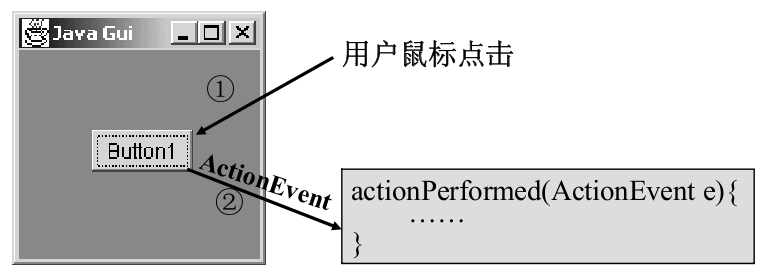
\includegraphics[width=0.8\textwidth]{fig10.png}
\end{figure}
\end{frame}

\begin{frame}[fragile] % [fragile]参数使得能够插入代码
\frametitle{事件处理相关概念}

\begin{description}[<+-|alert@+>]
\item[事件(Event)] 一个事件类型的对象,用于描述了发生什么事情,当用户在组件上进行操作时
  会触发相应的事件。
\item[事件源(Event Source)] 能够产生事件的GUI组件对象,如按钮、文本框等。
\item[事件处理方法(Event Handler)] 能够接收、解析和处理事件类对象,实现与用户交互功能的
  方法。
\item[事件监听器(Event Listener)] 调用事件处理方法的对象。
\end{description}

\codeset{sample.awt.event.ActionEventSample.java}

\end{frame}

\begin{frame}[fragile] % [fragile]参数使得能够插入代码
\frametitle{GUI事件类型层次}
\begin{figure}
\centering
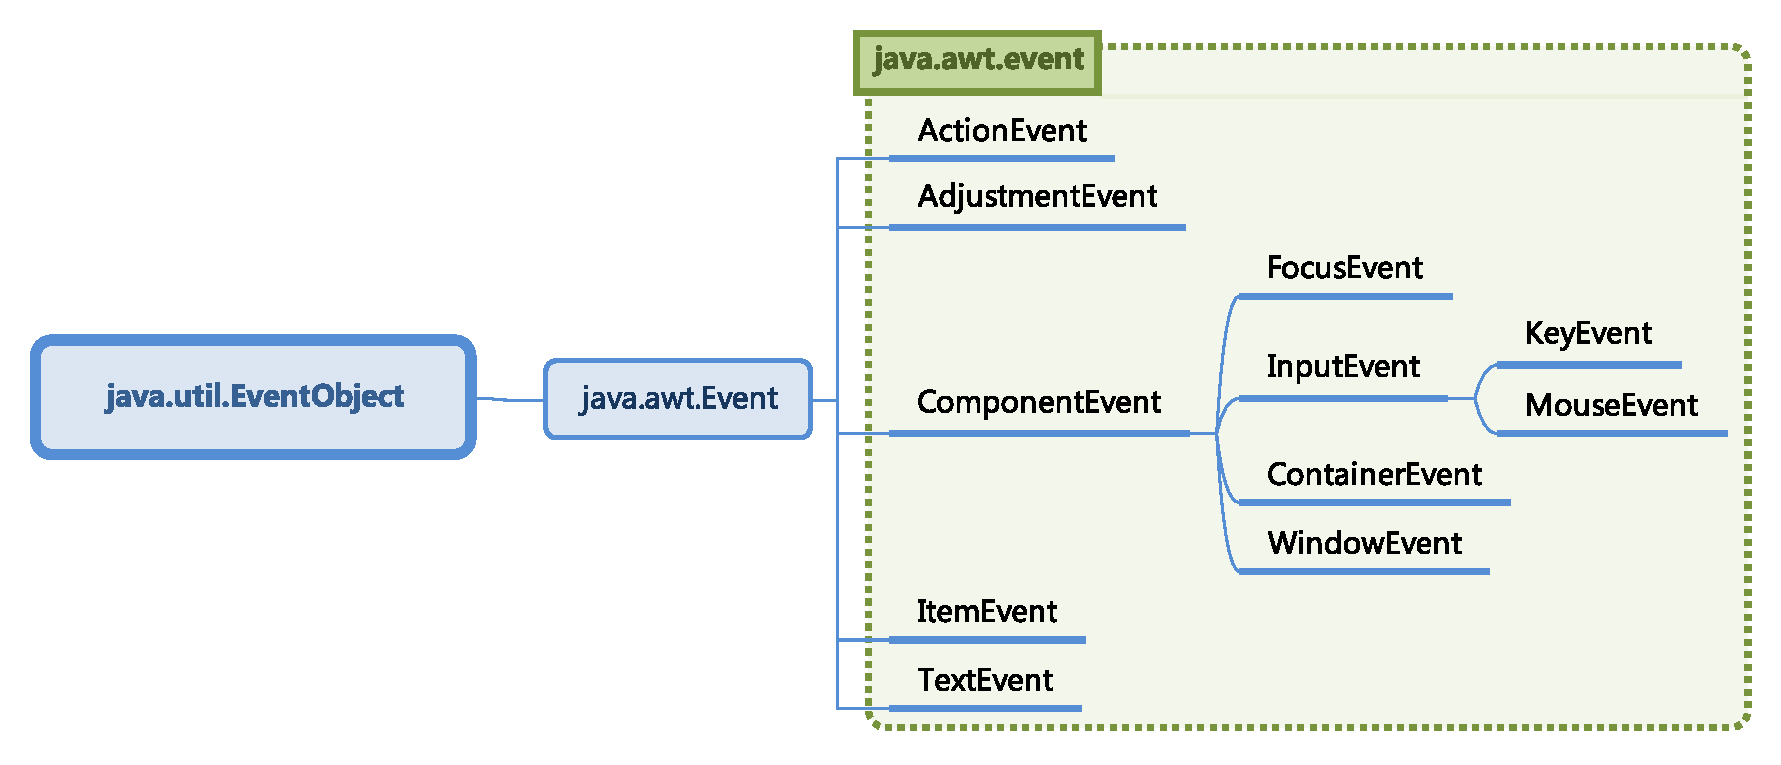
\includegraphics[width=\textwidth]{fig-awt-events.pdf}
\end{figure}
\end{frame}

\begin{frame}[fragile] % [fragile]参数使得能够插入代码
  \frametitle{GUI事件及相应监听器接口}
  \begin{table}
    \scriptsize
    \setlength{\extrarowheight}{1.2mm}
    \rowcolors[]{1}{blue!30}{blue!10}
    \begin{tabular}{lll}
      {\bf 事件类型} & {\bf 相应监听器接口} & {\bf 监听器接口中的方法}\\
      Action & ActionListener & actionPerformed(ActionEvent)\\
      Item & ItemListener & itemStateChanged(ItemEvent)\\
      Mouse & MouseListener & mousePressed(MouseEvent) ...\\
      MouseMotion & MouseMotionListener & mouseDragged(MouseEvent) ...\\
      Key & KeyListener & keyPressed(KeyEvent)\\
      Focus & FocusListener & focusGained(FocusEvent)\\
      Adjustment & AdjustmentListener & adjustmentValueChanged(AdjustmentEvent)\\
      Component & ComponentListener & componentMoved(ComponentEvent) ...\\
      Window & WindowListener & windowClosing(WindowEvent) ...\\
      Container & ContainerListener & componentAdded(ContainerEvent) ...\\
      Text & TextListener & textValueChanged(TextEvent) ...\\
    \end{tabular}
  \end{table}
\end{frame}

\begin{frame}[fragile] % [fragile]参数使得能够插入代码
  \frametitle{多重事件监听器}

  \begin{itemize}
  \item 一般情况下,事件源可以产生多种不同类型的事件,因而可以注册(触
    发)多种不同类型的监听器。
  \item 一个事件源组件上可以注册多个监听器,针对同一个事件源的同一种事
    件也可以注册多个监听器,一个监听器可以被注册到多个不同的事件源上。
  \end{itemize}

  \codeset{sample.awt.event.MulitActionsEventSample.java}
\end{frame}

\begin{frame}[fragile] % [fragile]参数使得能够插入代码
  \frametitle{事件适配器}

  \begin{itemize}[<+-|alert@+>]
  \item 当创建事件监听器类时,需要实现相应的监听器接口,而实现类中又必
    须重写/实现接口中的每一个抽象方法,这在GUI事件处理过程中经常会成为
    一种负担。
  \item 事件适配器使用了设计模式中的缺省适配器(Default Adapter)。事件
    适配器类(Adapter)是针对大多数事件监听器接口定义的相应抽象类,适
    配器类实现了相应监听器接口中所有的方法,但不做任何事。
  \end{itemize}

\codeset{sample.awt.event.EventAdapterSample.java}
\end{frame}

\begin{frame}[fragile] % [fragile]参数使得能够插入代码
  \frametitle{事件适配器}
  \tta{常用的GUI事件适配器}

  \begin{table}
    \scriptsize
    \setlength{\extrarowheight}{1.2mm}
    \rowcolors[]{1}{blue!30}{blue!10}
    \begin{tabular}{lll}
      {\bf 监听器接口} & {\bf 对应适配器类} & {\bf 说明}\\
      MouseListener & MouseAdapter & 鼠标事件适配器\\
      MouseMotionListener & MouseMotionAdapter & 鼠标运动事件适配器\\
      WindowListener & WindowAdapter & 窗口事件适配器\\
      FocusListener & FocusAdapter & 焦点事件适配器\\
      KeyListener & KeyAdapter & 键盘事件适配器\\
      ComponentListener & ComponentAdapter & 组件事件适配器\\
      ContainerListener & ContainerAdapter & 容器事件适配器\\
    \end{tabular}
  \end{table}
  
\end{frame}


%%%\begin{frame}[fragile]
%%%  \frametitle{内部类和匿名类在GUI事件处理中的应用}
%%%
%%%  监听器类中封装的业务逻辑具有非常强的针对性,一般没有重用价值,因此经
%%%  常采用内部类或匿名类的形式来实现。
%%%
%%%  \ttc{在GUI事件处理中使用内部类}
%%%  
%%%  \begin{javaCode}
%%%    public class TestInner {
%%%      // ... ...
%%%      private class InnerMonitor implements MouseMotionListener, MouseListener {// 内部类
%%%        public void mouseDragged(MouseEvent e) {
%%%          String s = "鼠标移动到位置 (" + e.getX() + ", " + e.getY() + ")");
%%%          tf.setText();
%%%        }
%%%        public void mouseEntered(MouseEvent e) {
%%%          String s = "鼠标已进入窗体";
%%%          tf.setText();
%%%        }
%%%        public void mouseExited(MouseEvent e) {
%%%          String s = "鼠标已移出窗体";
%%%          tf.setText();
%%%        }
%%%        public void mouseMoved(MouseEvent e) {}
%%%        public void mousePressed(MouseEvent e) {}
%%%        public void mouseClicked(MouseEvent e) {}
%%%        public void mouseReleased(MouseEvent e) {}
%%%      }
%%%      // ... ...
%%%    }
%%%  \end{javaCode}
%%%\end{frame}
%%%
%%%\begin{frame}[fragile]
%%%  \frametitle{内部类和匿名类在GUI事件处理中的应用}
%%%
%%%  如果不使用内部类实现上述代码?需要如何修改事件监听器类?
%%%
%%%  \ttc{使用外部类}
%%%  \begin{javaCode}
%%%    public class TestOuter {
%%%      ...
%%%      OurterMonitor om = new OutMonitor(tf);  // 将组件作为参数传递
%%%    }
%%%
%%%    class OuterMonitor implements MouseMotionListener, MouseListener { // 外部类
%%%      public OuterMonitor(TextField tf) { // 接收需要该类修改的外部组件对象
%%%        this.tf = tf;
%%%      }
%%%      public void mouseDragged(MouseEvent e) {
%%%        String s = "鼠标移动到位置 (" + e.getX() + ", " + e.getY() + ")");
%%%        tf.setText();
%%%      }
%%%      public void mouseEntered(MouseEvent e) {
%%%        String s = "鼠标已进入窗体";
%%%        tf.setText();
%%%      }
%%%      public void mouseExited(MouseEvent e) {
%%%        String s = "鼠标已移出窗体";
%%%        tf.setText();
%%%      }
%%%      public void mouseMoved(MouseEvent e) {}
%%%      // ... ...
%%%    }
%%%    // ... ...
%%%  }  
%%%\end{javaCode}
%%%\end{frame}

\begin{frame}[fragile] % [fragile]参数使得能够插入代码
  \frametitle{内部类和匿名类在GUI事件处理中的应用}

  监听器类中封装的业务逻辑具有非常强的针对性,一般没有重用价值,因此经常
  采用内部类或匿名类的形式来实现。

  \notice{一起改一改}

  \codeset{sample.awt.layout.CardLayoutSample.java}
  
  请同学将上述代码中的窗口事件监听代码修改为匿名类形式。

%%%  \tta{使用匿名类}
%%%
%%%  \begin{javaCode}
%%%    // ... ...
%%%    f.addWindowListener(new WindowAdapter() { // 定义匿名类
%%%      public void windowClosing(WindowEvent e) {
%%%        System.exit(0);
%%%      }
%%%    });
%%%    // ... ...
%%%  \end{javaCode}
\end{frame}

\section{Applet}

\begin{frame}[fragile] % [fragile]参数使得能够插入代码
  \frametitle{Applet}

  \tta{Applet,昔日的互联网野心!}
  
  Applet也称Java小程序,在支持Java的浏览器环境中运行,通常用于在网页中实现嵌入图片、播放声
  音等多媒体功能,或添加其他的客户端处理逻辑(如网络计算器)。

  {\hei 严格的说,Applet是能够嵌入到HTML页面中,且可以通过Web浏览器下载并执行的一种Java程序。}

  目前,该项技术在新项目中已经很少使用。

\end{frame}

\begin{frame}[fragile] 
  \frametitle{Applet生命周期}

  \begin{figure}
    \centering
    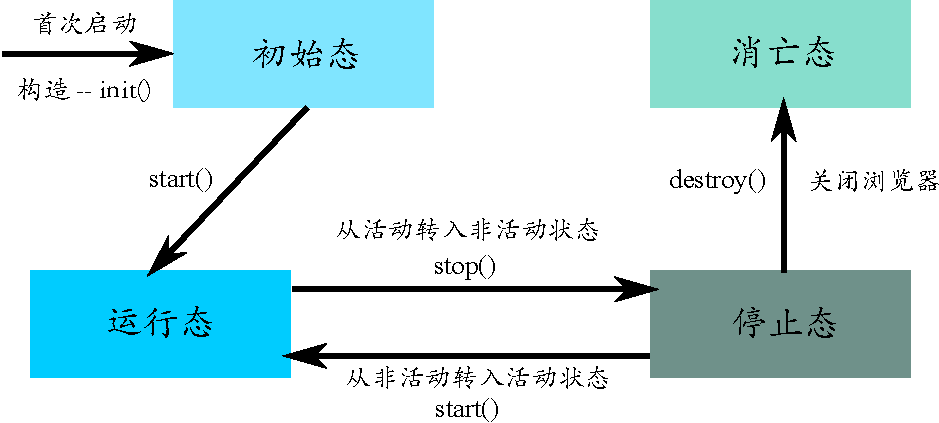
\includegraphics[width=0.8\textwidth]{figures/fig05.pdf}
  \end{figure}
\end{frame}


\begin{frame}[fragile] 
  \frametitle{Applet示例}

  \samp{GoodbyeApplet.java}
  
  \begin{javaCode}
    import java.applet.Applet;
    import java.awt.Color;
    import java.awt.Graphics;

    public class HelloApplet extends Applet {
      String text;
      public void init() {
        text = "Hello Applet, goodbye!";
        this.setBackground(new Color(120, 180, 140));
      }
      public void paint(Graphics g) {
        g.drawString(text, 25, 25);
      }
    }
  \end{javaCode}

  \samp{test.html}
  
  \begin{shCode}
    <html>
    <applet code="HelloApplet.class" width=200 height=150> </applet>
    </html>  
  \end{shCode}

  可以使用Applet viewer小工具运行示例:
  
  \begin{shCode}
    >appletviewer test.html
  \end{shCode}
\end{frame}

%%%%%%%%%%%%%%%%%%%%%%%%%%%%%%%%%%%%%%%%%%%%%%%%%%
\section{Swing}

\begin{frame}[fragile] % [fragile]参数使得能够插入代码
  \frametitle{Swing概述}

  \tta{Swing与AWT的关系}

  Swing是建立在AWT基础上的一种增强型Java GUI组件和工具集
  \begin{itemize}\kai
  \item 使用轻量组件以替代AWT中的绝大部分重量组件。
  \item 提供AWT所缺少的一些附件组件和观感控制机制。
  \item 提供更好的平台无关性。
  \end{itemize}

  \tta{相关基本概念}
  \ttc{Java基础类库(Java Foundation Classes, JFC)}\\
  Java基础类库是用于图形用户界面开发的Java API集,具体包括AWT、2D API、Swing组件
  和Accessibility API。
\end{frame}

\begin{frame}[fragile] % [fragile]参数使得能够插入代码
  \frametitle{Swing概述}
  \ttc{重量组件(Heavy-Weight Components)}\\
  \begin{itemize}
  \item 重量组件通过委托对等组件(对等组件指底层平台,如Windows操作系统的用户界面组件)来完
    成具体工作,包括组件的绘制和事件响应。AWT中的组件均为重量组件,或者说,AWT组件只是对本
    地对等组件的封装。
  \item 开销大、效率低、无法实现组件的“透明”效果。
  \end{itemize}
\end{frame}

\begin{frame}[fragile] % [fragile]参数使得能够插入代码
  \frametitle{Swing概述}

  \ttc{轻量组件(Light-Weight Components)}\\
  \begin{itemize}
  \item 轻量组件不存在本地对等组件,通过Java绘图技术在其所在的容器窗口中绘图得到。
  \item 能够实现组件的透明效果,能够做到不同平台上的一致表现。
  \item 组件绘制和事件处理机制的开销小。
  \item 轻量组件最终需要包含在一个重量容器中。因此,Swing组件中的几个顶层容器(如JFrame、
    JDialog和JApplet)采用了重量组件,其余的均为轻量组件。
  \item 不建议轻重组件混用。
  \end{itemize}
\end{frame}

\begin{frame}[fragile] % [fragile]参数使得能够插入代码
  \frametitle{Swing概述}
  \ttc{可视化组件(Visual Component)}

  \begin{itemize}
  \item 和AWT组件类似,Swing组件也分为可视化和非可视化组件。
  \item 可视化组件为能够显示特定形状、颜色和尺寸的组件;非可视化组件也称支持类,如布局管理
    器等。
  \item Swing可视化组件类名均以J开头。
  \end{itemize}
\end{frame}

\section{Swing典型组件(课后自学)}

\begin{frame}[fragile] % [fragile]参数使得能够插入代码
  \frametitle{JFrame}
  \begin{enumerate}
  \item JFrame继承并扩充了java.awt.Frame类。\\
    {\kai JFrame不再是一个单一容器,而是由相互间存在包含关系的多个不同容器面
      板(JRootPane, GlassPane, LayeredPane, ContentPane)组成,我们实际上只使用其中的内容
      面板(ContentPane)。}
  \item JFrame实现了javax.swing.WindowConstants接口,该接口中定义了用于控制窗口关闭操作的整型
    常量,包括:
    \begin{itemize}\small
    \item DO\_NOTHING\_ON\_CLOSE
    \item HIDE\_ON\_CLOSE
    \item DISPOSE\_ON\_CLOSE
    \item EXIT\_ON\_CLOSE
    \end{itemize}
  \end{enumerate}
\end{frame}

\begin{frame}[fragile] % [fragile]参数使得能够插入代码
  \frametitle{JFrame示例}
  \samp{TestJFrame.java}
  \begin{javaCode}
    import java.awt.Color;
    import java.awt.Container;
    import java.awt.FlowLayout;
    import javax.swing.JFrame;
    import javax.swing.JLabel;

    public class TestJFrame {
      public static void main(String[] args){
        JFrame jf = new JFrame("My Test");
        Container c = jf.getContentPane(); 
        c.setLayout(new FlowLayout(FlowLayout.LEFT, 20, 20));
        JLabel greet = new JLabel("Hello, World!");
        JLabel bye = new JLabel("Bye, World!");
        bye.setBackground(Color.BLUE);
        bye.setOpaque(true); // 设置为不透明
        c.add(greet);
        c.add(bye);
        c.setBackground(Color.GREEN);
        jf.setSize(400, 300);
        jf.setLocation(400, 200);
        jf.setDefaultCloseOperation(JFrame.EXIT_ON_CLOSE); // 等同于显示注册 WindowListener
        jf.setVisible(true);
      }
    }
  \end{javaCode}
\end{frame}

\begin{frame}[fragile] % [fragile]参数使得能够插入代码
  \frametitle{JFrame}

  为了方便开发,从JDK5.0开始JFrame类重写了其add()、remove()和setLayout()方法,这些重写后的方法{\hei 将针对JFrame的添加组件、移除组件和设置布局管理器等操作自动转发给其内容面板contentPane,以实现对contentPane的直接控制}。

  对上述代码的改写:

  \begin{javaCode}
    JFrame jf = new JFrame("My Test");
    jf.setLayout(new FlowLayout(FlowLayout.LEFT, 20, 20));
    JLabel greet = new JLabel("Hello, World!");
    jf.add(greet);
    jf.getContentPane().setBackground(Color.GREEN); // 注意
  \end{javaCode}

  {\Red\kai 注意:setBackground()方法在JFrame类中并没有进行重写,因此不会将针对JFrame的颜色设置操作自动转发到其内容面板。}
\end{frame}

\begin{frame}[fragile] % [fragile]参数使得能够插入代码
  \frametitle{Swing按钮、菜单和工具条}

  \begin{itemize}
  \item JButton\\
    能够实现更复杂的显式效果,例如可以使用图片作为按钮标签、设置快捷键和添加工具提示信息。
  \item 菜单\\
    同样分为菜单条、菜单和菜单项(JMenuBar、JMenu、JMenuItem),用法与AWT完全相同。
  \item 工具条\\
    工具条是用于显示常见组件的条形容器,一般用法是向工具条中添加一系列
    图标形式的按钮,并将之置于窗口上方边缘。{\kai 例如,BorderLayout布
      局的北部区域,对于大多数的外观,用户可以用鼠标直接将工具栏拖
      到BorderLayout布局的其他未添加组件的边缘区域,如西部或东部,也可
      以将之拖出到单独的窗口中显示。}
  \end{itemize}
\end{frame}

\begin{frame}[fragile] % [fragile]参数使得能够插入代码
  \frametitle{Swing按钮、菜单和工具条}

  \samp{TestSwing.java}

  \scriptsize
\begin{verbatim}
import java.awt.event.*;
import javax.swing.*;

public class TestSwing implements ActionListener {
  public static void main(String[] args) {
    new TestSwing().createUI();
  }

  public void createUI() {
    JFrame jf = new JFrame("Test Swing");
    JMenuBar jmb = new JMenuBar();
    JMenu menu_file = new JMenu("File");
    JMenu menu_help = new JMenu("Help");
    JMenuItem mi_new = new JMenuItem("New");
    JMenuItem mi_open = new JMenuItem("Open");
    JMenuItem mi_save = new JMenuItem("Save");
    mi_new.addActionListener(this);
    mi_open.addActionListener(this);
    mi_save.addActionListener(this);
\end{verbatim}
\end{frame}

\begin{frame}[fragile] % [fragile]参数使得能够插入代码
\frametitle{Swing按钮、菜单和工具条}
\scriptsize
\begin{verbatim}    
    mi_new.setMnemonic('N');
    mi_open.setMnemonic('O');
    mi_save.setMnemonic('S');
    menu_file.setMnemonic('F');
    menu_help.setMnemonic('h');
    
    menu_file.add(mi_new);
    menu_file.add(mi_open);
    menu_file.add(mi_save);
    
    jmb.add(menu_file);
    jmb.add(menu_help);

    JToolBar jtb = new JToolBar();
    JButton button_new = new JButton("NEW");
    JButton button_open = new JButton("OPEN");
    JButton button_save = new JButton("SAVE");

    button_new.setActionCommand("New");
    button_open.setActionCommand("Open");
    button_save.setActionCommand("Save");
\end{verbatim}
\end{frame}

\begin{frame}[fragile] % [fragile]参数使得能够插入代码
\frametitle{Swing按钮、菜单和工具条}
\scriptsize
\begin{verbatim}
    button_new.setToolTipText("Create a new file");
    button_open.setToolTipText("Open the file");
    button_save.setToolTipText("Save the file");
    
    button_new.addActionListener(this);
    button_open.addActionListener(this);
    button_save.addActionListener(this);
    
    jtb.add(button_new);
    jtb.add(button_open);
    jtb.add(button_save);
    
    JPanel jp = new JPanel();
    JButton button_start = new JButton("Start");
    JButton button_stop = new JButton("Stop");
    button_start.addActionListener(this);
    button_stop.addActionListener(this);
    jp.add(button_start);
    jp.add(button_stop);
\end{verbatim}
\end{frame}

\begin{frame}[fragile] % [fragile]参数使得能够插入代码
\frametitle{Swing按钮、菜单和工具条}
\scriptsize
\begin{verbatim}		
    jf.setJMenuBar(jmb); // Menu 不需要使用 add() 方法添加
    jf.add(jtb, "North");
    jf.add(jp, "South");
    
    jf.setSize(600, 400);
    jf.setLocation(400, 200);
    jf.setDefaultCloseOperation(JFrame.EXIT_ON_CLOSE);
    jf.setVisible(true);
  }

  @Override
  public void actionPerformed(ActionEvent e) {
    System.out.println(e.getActionCommand());
  }
}  
\end{verbatim}
\end{frame}

\begin{frame}[fragile] % [fragile]参数使得能够插入代码
\frametitle{标准对话框}

使用标准对话框(JOptionPane)可以实现程序与用户的便捷交互,如向用户发送错误通知、警告/确
认用户操作、接收用户输入或选择的简单信息等。

\samp{示例}
\scriptsize
\begin{verbatim}
  @Override
  public void actionPerformed(ActionEvent e) {
    String s = e.getActionCommand();
    if (s.equals("Error")) {
      JOptionPane.showMessageDialog(null, "这是一个错误提示对话框", "错误提示",
      JOptionPane.ERROR_MESSAGE);
    } else if (s.equals("Confirm Quit")) {
      int result = JOptionPane.showConfirmDialog(null, "真的要退出程序么?",
      "请确认退出", JOptionPane.YES_NO_OPTION);
      if (result == JOptionPane.OK_OPTION) {
        System.exit(0);
      }
\end{verbatim}
\end{frame}

\begin{frame}[fragile] % [fragile]参数使得能够插入代码
\frametitle{标准对话框}

\scriptsize
\begin{verbatim}
    } else if (s.equals("Warning")) {
      Object[] options = { "继续", "撤销" };
      int result = JOptionPane.showOptionDialog(null, "本操作可能导致数据丢失",
      "警告", JOptionPane.DEFAULT_OPTION,
      JOptionPane.WARNING_MESSAGE, null, options, options[0]);
      if (result == 0)
        System.out.println("继续操作");
    } else if (s.equals("Input")) {
      String name = JOptionPane.showInputDialog("请输入姓名:");
      if (name != null) 
        System.out.println("输入的姓名为" + name);
    } else if (s.equals("Choice")) {
      Object[] possibleValues = { "体育", "政治", "经济", "文化" };
      Object selectedValue = JOptionPane.showInputDialog(null,
      "Choice one", "Input", JOptionPane.INFORMATION_MESSAGE,
      null, possibleValues, possibleValues[0]);
      String result = (String) selectedValue;
      if (result != null) 
        System.out.println("你的选择是:" + result);
    }
  }
\end{verbatim}
\end{frame}

\begin{frame}[fragile] % [fragile]参数使得能够插入代码
\frametitle{表格和树}
\begin{itemize}
\item {\bf javax.swing.JTable}\\
用于以传统的表格形式来显示数据,通过注册监听器的方式关联响应的处理逻辑。
\begin{itemize}
\item 表头:标题行,给出每一列(字段)的名称。
\item 表体:由多行多列、规则矩阵形式的单元格组成,真正的数据信息则显示在每个单元格中。
\end{itemize}
\item {\bf javax.swing.JTree}\\
以树状结构分层次显示数据信息,例如操作系统提供的资源管理器。
\end{itemize}
\end{frame}

\begin{frame}[fragile] % [fragile]参数使得能够插入代码
\frametitle{表格示例}

\begin{columns}
\column{0.4\textwidth}  
\tta{表格}
\begin{figure}
\centering
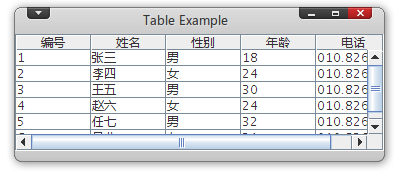
\includegraphics[width=0.95\textwidth]{swing-fig01.png}
\end{figure}

\column{0.6\textwidth}  
\begin{javaCode}
import java.awt.event.WindowAdapter;
import java.awt.event.WindowEvent;
import javax.swing.JFrame;
import javax.swing.JScrollPane;
import javax.swing.JTable;
public class TableExample {
  public static void main(String[] args) {
    JFrame myFrame = new JFrame("Table Example");
    Object data[][] = {
      {1, "张三", "男", "18", "010.82607080"},
      {2, "李四", "女", "24", "010.82607080"},
      {3, "王五", "男", "30", "010.82607080"},
      // ... ...
    };
    String columnNames[] = {
      "编号", "姓名", "性别", "年龄", "电话"};
    JTable table = new JTable(data, columnNames);
    table.setAutoResizeMode(JTable.AUTO_RESIZE_OFF);
    JScrollPane pane = new JScrollPane(table);
    myFrame.add("Center", pane);
    myFrame.setSize(450, 250);
    myFrame.addWindowListener(new WindowAdapter(){
      public void windowClosing(WindowEvent e) {
        System.exit(0);
      }
    });
    myFrame.setVisible(true);
  }
}
\end{javaCode}
\end{columns}
\end{frame}

\begin{frame}[fragile] % [fragile]参数使得能够插入代码
\frametitle{表格其他参考例程}
\begin{enumerate}
\item A Simple Interactive JTable Tutorial\\
http://www.javalobby.org/articles/jtable/
\end{enumerate}

\end{frame}
\begin{frame}[fragile] % [fragile]参数使得能够插入代码
\frametitle{树示例}

\tta{树}
\begin{figure}
\centering
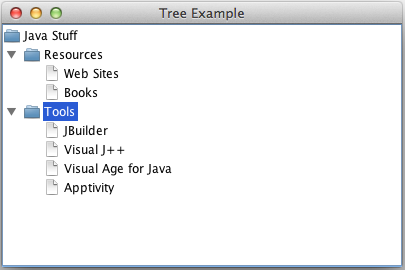
\includegraphics[width=0.6\textwidth]{swing-fig02.png}
\end{figure}

\end{frame}

\begin{frame}[fragile] % [fragile]参数使得能够插入代码
\frametitle{树示例}

\samp{TreeExample.java}

\begin{javaCode}
public class TreeExample {
  public static DefaultMutableTreeNode createNodes() {
    DefaultMutableTreeNode rootNode = new DefaultMutableTreeNode("Java Stuff");
    DefaultMutableTreeNode resources = new DefaultMutableTreeNode("Resources");
    DefaultMutableTreeNode tools = new DefaultMutableTreeNode("Tools");
    rootNode.add(resources);
    rootNode.add(tools);
    DefaultMutableTreeNode webSites = new DefaultMutableTreeNode("Web Sites");
    DefaultMutableTreeNode books = new DefaultMutableTreeNode("Books");
    resources.add(webSites);
    resources.add(books);
    tools.add(new DefaultMutableTreeNode("JBuilder"));
    tools.add(new DefaultMutableTreeNode("Visual J++"));
    return rootNode;
  }
  public static void main(String[] args) {
    JFrame myFrame = new JFrame("Tree Example");
    DefaultMutableTreeNode rootNode = createNodes();
    JTree tree = new JTree(rootNode);
    tree.setRootVisible(true);
    JScrollPane pane = new JScrollPane();
    pane.setViewportView(tree);
    myFrame.add(pane, "Center");
    myFrame.setSize(400, 250);
    myFrame.setDefaultCloseOperation(JFrame.EXIT_ON_CLOSE);
    myFrame.setVisible(true);
  }
}
\end{javaCode}
\end{frame}

\begin{frame}[fragile] % [fragile]参数使得能够插入代码
\frametitle{JTable和JTree的MVC模式}

JTable和JTree采用了相对独立的方式向组件提供要显示的数据,即当显示/处理的数据结构较复杂
时,将GUI组件结构分为相对独立的{\hei 模型、视图、控制器}三个模块,模块间存在专门的分工和
协作关系。
\begin{enumerate}\kai 
\item {\hei 模型(Model)} 维护数据并提供数据访问方法,即数据和数据的处理逻辑。
\item {\hei 视图(View)} 绘制模型的视觉表现,即显示数据。视图就是用户能够看到并与之进行
  交互的用户界面。
\item {\hei 控制器(Controllor)} 负责处理事件或者说程序的流程控制,接受用户输入,并调
  用/操控模型和视图以实现用户需求。
\end{enumerate}
\end{frame}

\begin{frame}[fragile] % [fragile]参数使得能够插入代码
\frametitle{MVC作用原理}

\begin{figure}
\centering
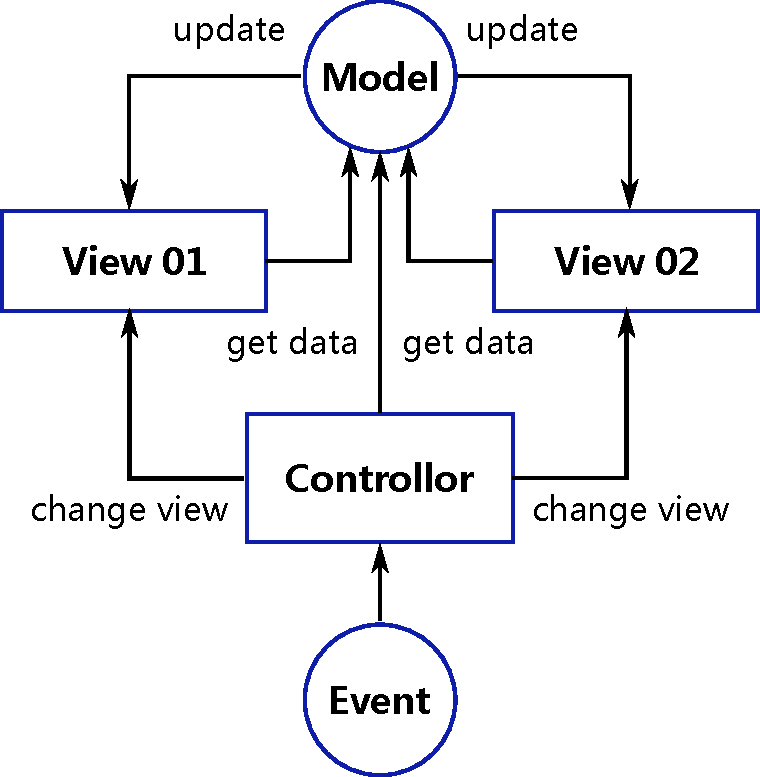
\includegraphics[width=0.5\textwidth]{swing-fig02.pdf}
\end{figure}
\end{frame}

\begin{frame}[fragile] % [fragile]参数使得能够插入代码
\frametitle{定时器}

javax.swing.Timer提供了定时器功能,用于在指定的时间延迟之后触发ActionEvent事件,以执行所
需的处理逻辑。

{\kai 具体的做法是:首先创建Timer对象,并在其上注册一个或多
  个ActionListener类型的监听器,在监听器事件处理方法actionPerformed()中
  应以实现给出要延时执行的任务代码,然后调用Timer对象的start()方法启动
  定时器即可。}

\tta{相关方法} 
\begin{itemize}
\item setRepeats() 设置计时器的动作。
\item setInitialDelay() 设置首次延迟时间。
\item start() 开始计时器。
\item stop() 停止计时器。
\item restart() 恢复计时器。
\end{itemize}
\end{frame}

\begin{frame}
  \frametitle{本节习题}
  \begin{enumerate}
  \item 制作思维导图,梳理Java Swing GUI库中各组件功能及编程知识点,看
    看谁总结的好,做的漂亮。
  \item 自行了解Java FX,参考互联网公开资料写一个Sample Code出来。
  \end{enumerate}
\end{frame}
%%%%%%%%%%%%%%%%%%%%%%%%%%%%%%%%%%%%%%%%%%%%%%%%%%%%%%%%%%%%%%%%%%%%%%%%%%%%%%%
% TKS Page %%%%%%%%%%%%%%%%%%%%%%%%%%%%%%%%%%%%%%%%%%%%
\begin{frame}
\centering
{\Huge \textcolor{blue}{THE END}} \\
\vspace{5mm}
{\Large wangxiaodong@ouc.edu.cn} \\
\end{frame}
%%%%%%%%%%%%%%%%%%%%%%%%%%%%%%%%%%%%%%%%%%%%%%%%%%%%%%%
%%%%%%%%%%%%%%%%%%%%%%%%%%%%%%%%%%%%%%%%%%%%%%%%%%%%%%%%%%%%%%%%%%%%%%%%%%%%%%%
\end{document}

